\chapter{Anormale Diffusion - Lorentz-Modell}

\section{Lorentz-Modell}

Zum Abschluss soll das Diffusionsverhalten von Teilchen untersucht werden, die auf den Porenraum des Boolschen Modells beschr�nkt sind. Dieser spezielle Anwendungsfall wird auch als Lorentz-Modell bezeichnet. Die Visualisierung der Teilchentrajektorie eines Testteilchens mit Radius $\sigma = 0.1$ ist in \fref{fig:big} zu sehen.

\begin{figure}[!ht]
	\centering
		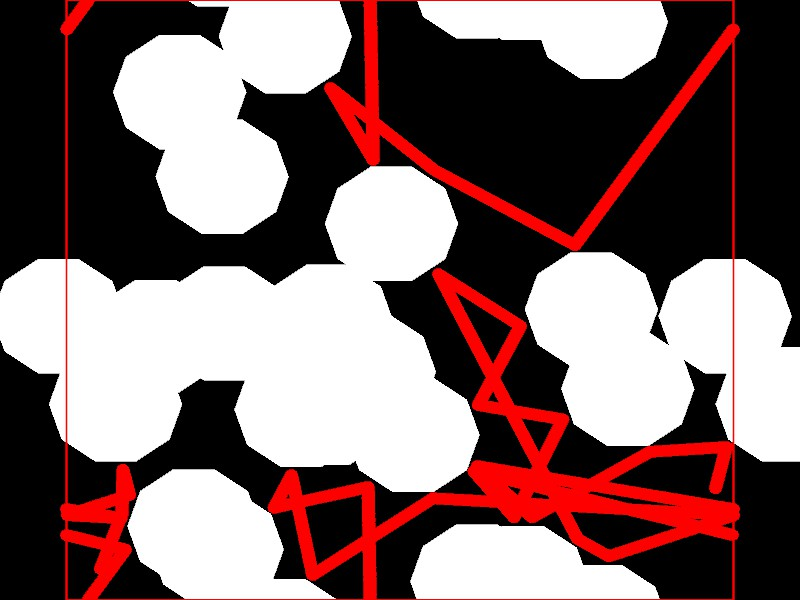
\includegraphics[width=0.70\textwidth]{img/big.jpg}
	\caption{Teilchentrajektorie im Porenraum des Boolschen Modells f�r ein Teilchen mit Radius $\sigma = 0.1$}
	\label{fig:big}
\end{figure}

Die erste Frage, die sich stellt, ist, ob sich die Trajektorie �ndert, wenn man Punktteilchen betrachtet und daf�r den Radius der Scheiben, die die Hindernisse darstellen, auf $R=R+\sigma$ vergr��ert. Da f�r die St��e mit den Hindernisteilchen vollkommen elastische St��e angenommen werden, f�hrt diese �nderung zu den gleichen Trajektorien (siehe \fref{fig:small}). Dies f�hrt zu folgender �quivalenz:
\begin{equation}
\label{eq:aquivalenz}
\left( R, \sigma \right) \Leftrightarrow \left( R + \sigma, 0  \right)
\end{equation}
Durch das gleiche Argument spielt auch der Betrag der Anfangsgeschwindigkeit der Teilchen keine Rolle. Die Teilchen legen zwar insgesamt f�r h�here Anfangsgeschwindigkeiten weitere Wege zur�ck, aber das Abprallverhalten an den Hindernisse bleibt das gleiche.

\begin{figure}[!ht]
	\centering
		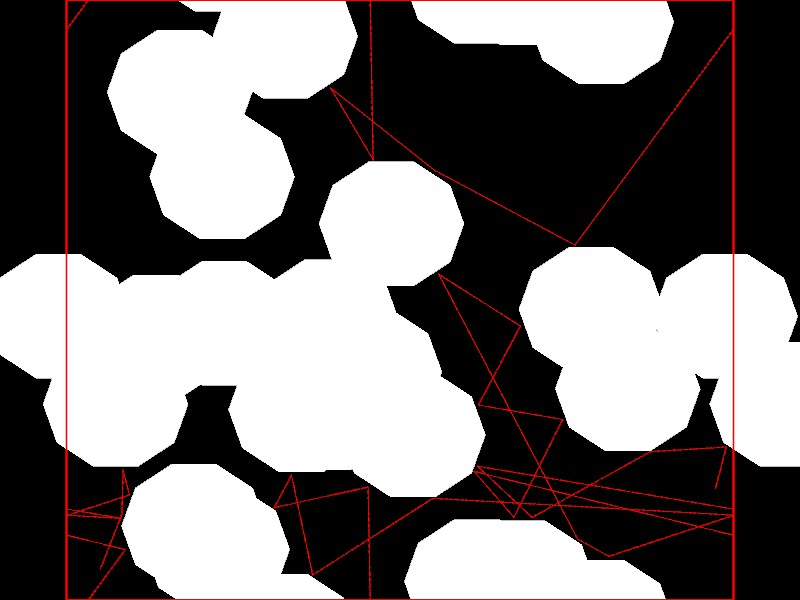
\includegraphics[width=0.70\textwidth]{img/small.jpg}
	\caption{Die Gr��e der Testteilchen spielt keine Rolle, wenn die Gr��e der Hindernisse angepasst wird (vgl \fref{fig:big}).}
	\label{fig:small}
\end{figure}

\section{Diffusionsverhalten}
F�r das Diffusionsverhalten im Lorentz-Modell ergeben sich nahe der Perkolationsschwelle interessante Ph�nomene. Zur Untersuchung dieses Verhaltens wird folgende Konfiguration verwendet.

\begin{figure}[!ht]
	\centering
		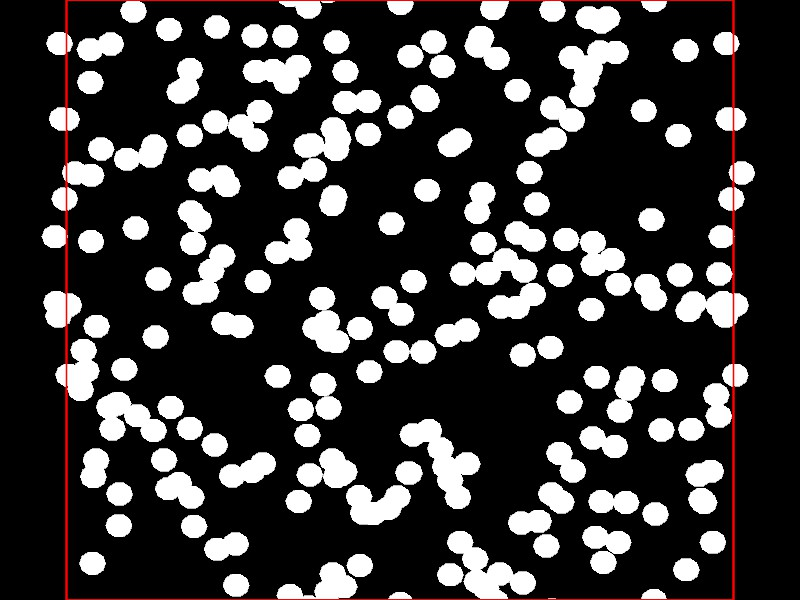
\includegraphics[width=0.70\textwidth]{img/lorentz.jpg}
	\caption{Testkonfiguration f�r die Diffusion im Lorentz-Modell.}
	\label{fig:lorentz}
\end{figure}

Um die Diffusionseigenschaften zu untersuchen wird jeweils �ber 100 Testteilchen gemittelt. Dieses Experiment wird f�r verschiedene Teilchenradien durchgef�hrt. Durch die in \fref{eq:aquivalenz} gegebene �quivalenz l�sst sich damit das verhalten nahe am Perkolationspunkt untersuchen. Der Perkolationspunkt des angegebenen Systems liegt bei (1.7562, 0).

\begin{figure}[!ht]
	\centering
		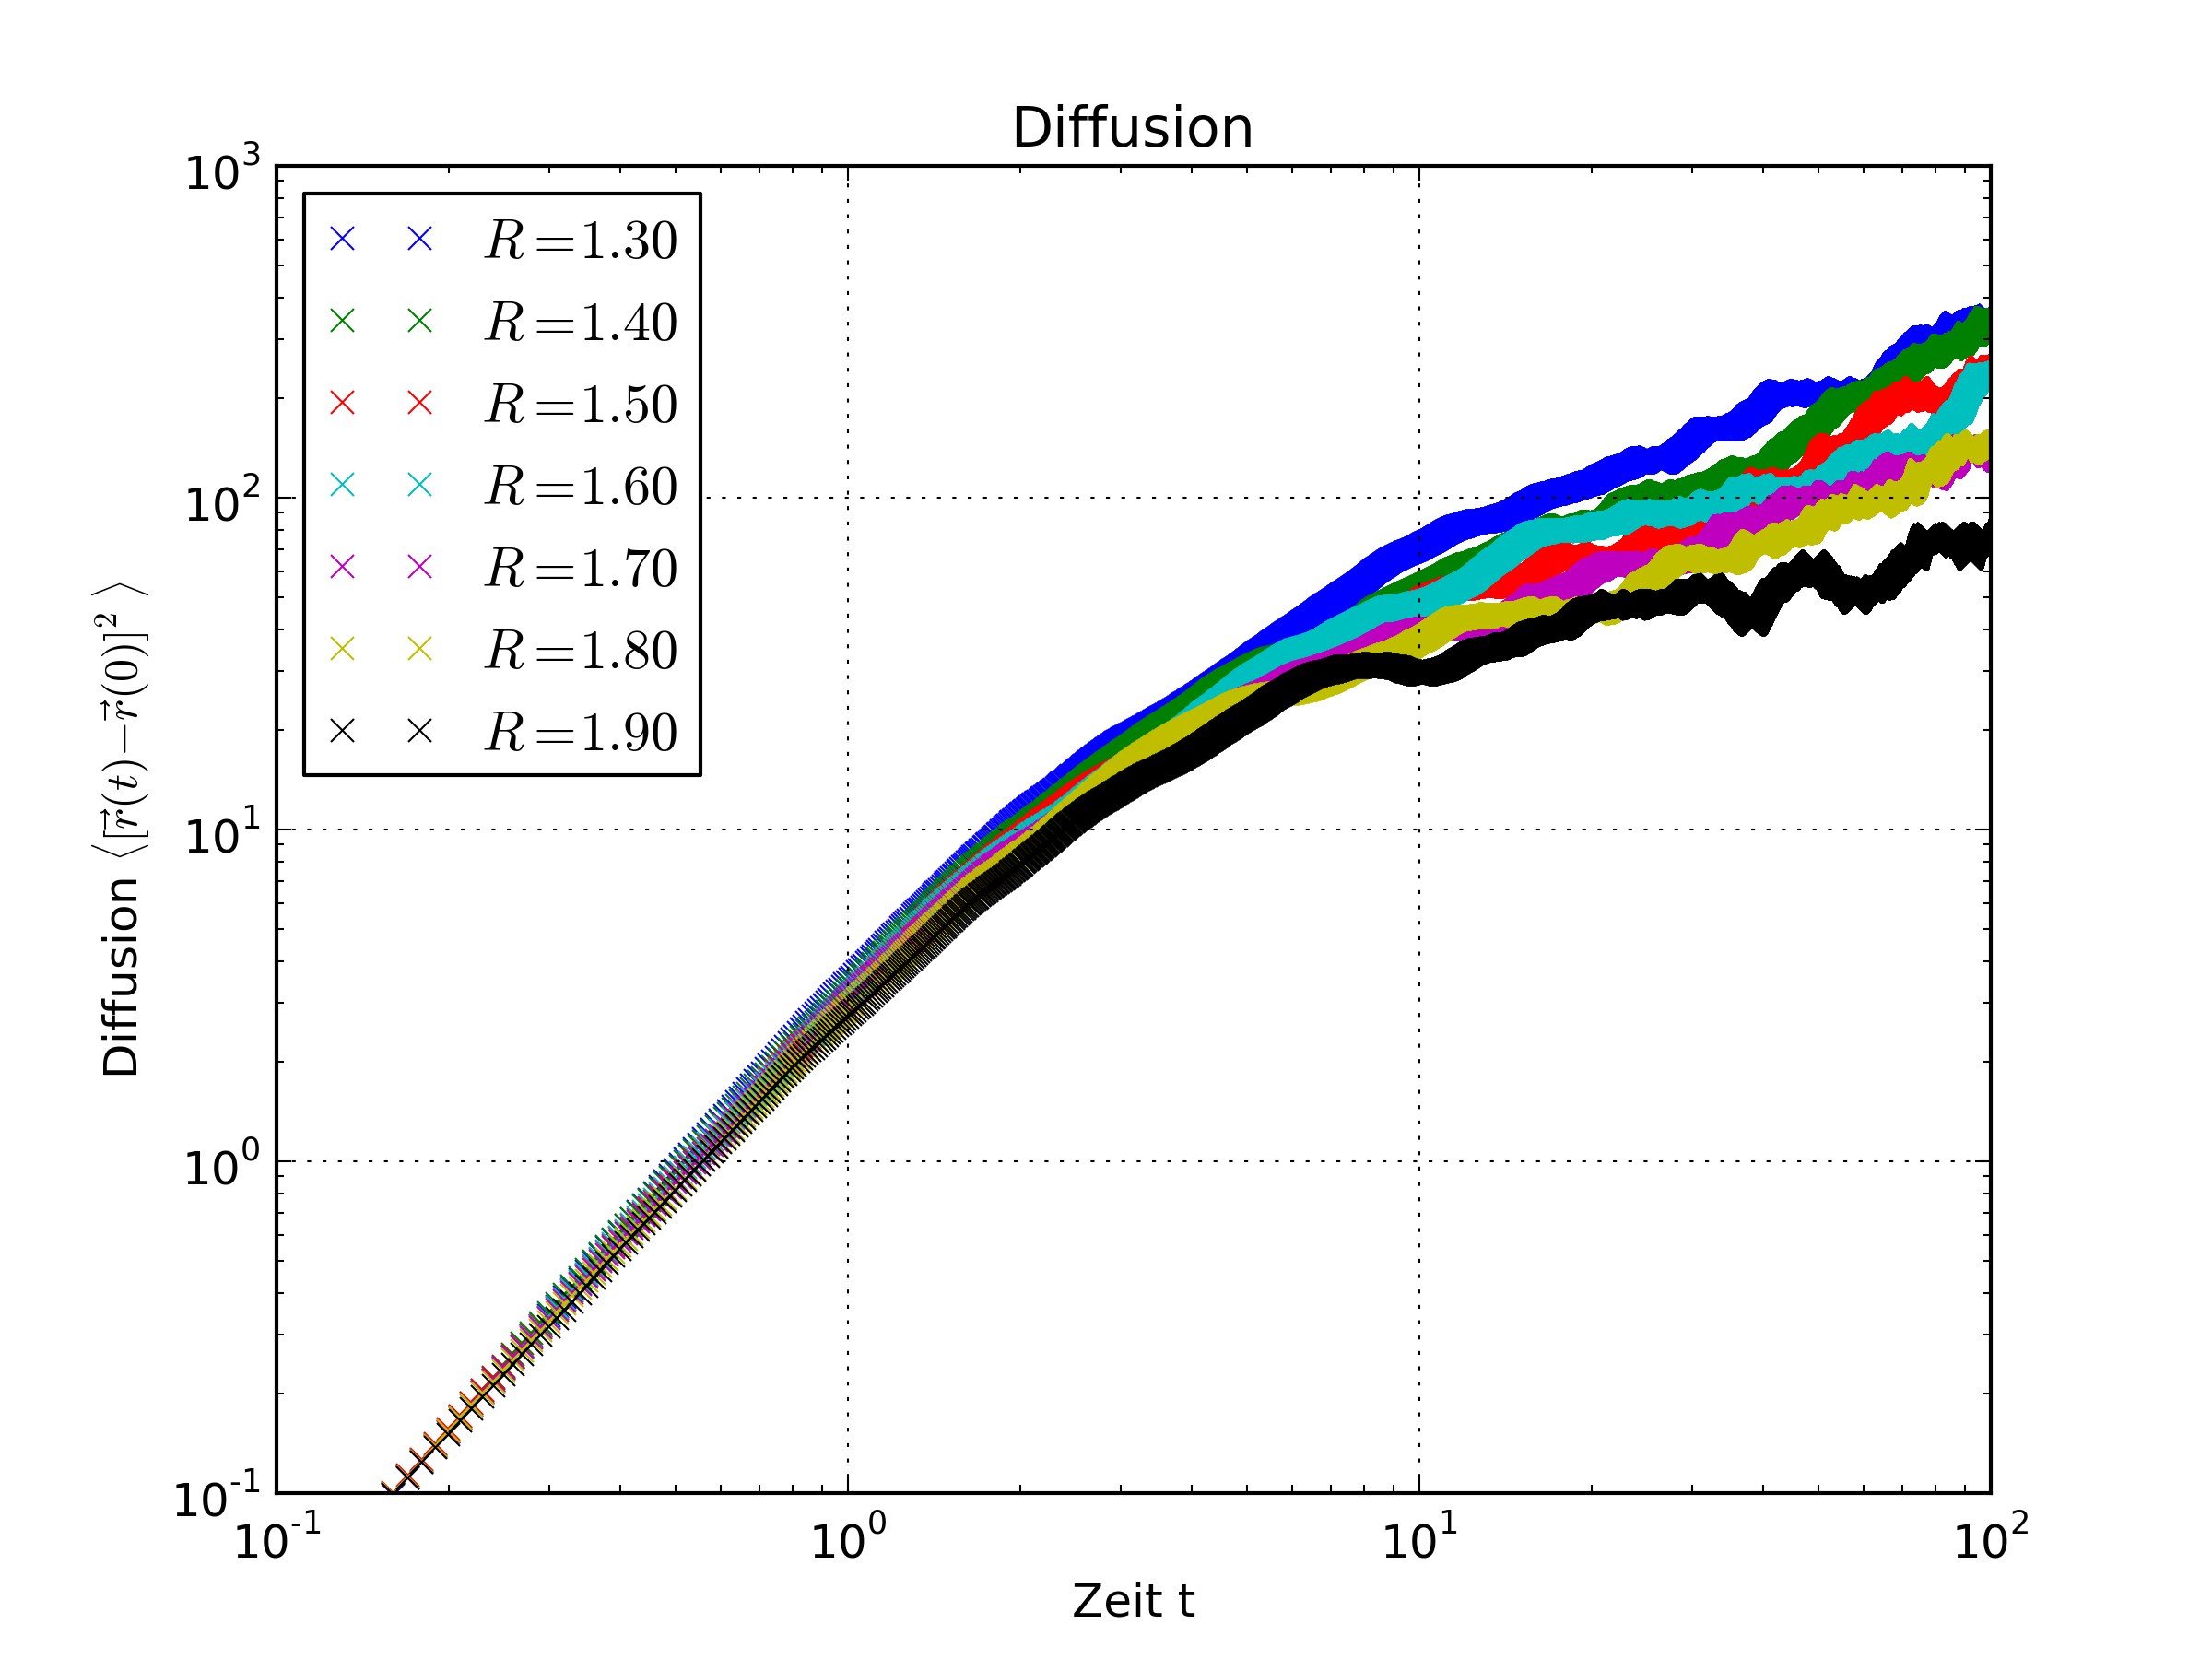
\includegraphics[width=0.70\textwidth]{img/A5_diffusion.png}
	\caption{Diffusionsverhalten bei verschieden gro�em Hindernisradius R. Die Testteilchen besitzen in dieser Darstellung einen Radius von $\sigma=0$. In der N�he der Perkolationsschwelle lassen sich Diffusionen mit einem exponenten zwischen 0 und 1 beobachten.}
	\label{fig:A5_diffusion}
\end{figure}

F�r kleinen Hindernisradius l�sst sich normales diffusives Verhalten mit einem Exponenten von 1 beobachten. F�r sehr gro�e Hindernisradien wird das Verhalten beschr�nkt (Exponent = 0). Im Bereich um den Perkolationspunkt lassen sich verschiedene andere Exponenten im Intervall [0,1] beobachten. Das Diffusionsverhalten mit Exponenten in diesem Bereich bezeichnet man als anormale Diffusion.